\subsection{Regulación variable con L78XX}
En un regulador con circuito integrado puede hacerse una variación en el pin de
tierra para variar el voltaje de salida, conectando dos resistencias
auxiliares.

En la \textbf{figura~\ref{circuito11}} se muestra el circuito regulador de
voltaje variable con un circuito integrado \textbf{L7809CV} que fija el voltaje
a $9[\text{V}]$ y con la ayuda de un potenciómetro de $1[\text{k}\Omega]$.

\begin{figure}[!h]
\centering
\includegraphics[scale=1.1]{diagramas/12.regulador4.eps}
\caption{Regulación de voltaje variable con \textbf{L7809CV}.}
\label{circuito11}
\end{figure}

Según la ley de mallas de \emph{Kirchhoff} a la salida del regulador se tiene:
\begin{equation*}
    \begin{split}
        V_{\text{out}} &= V_{\text{reg}} + I_2\,R_2\\
    \end{split}
\end{equation*}

Según la ley de nodos de \emph{Kirchhoff} a la salida del regulador se tiene:
\begin{equation*}
    \begin{split}
        I_2 &= \left(\frac{V_{\text{reg}}}{R_1} + I_Q\right)\\
    \end{split}
\end{equation*}

Por tanto:
\begin{equation*}
    \begin{split}
        V_{\text{out}} &= V_{\text{reg}} + R_2
        \left(\frac{V_{\text{reg}}}{R_1} + I_Q\right)\\
    \end{split}
\end{equation*}

La variación del voltaje de salida varia desde $9[\text{V}]$ para un valor de
$0[\Omega]$ en la resistencia variable, hasta el máximo que provee el
rectificador para el valor de $1[\text{k}\Omega]$.

\subsubsection{Simulación}
Se utilizó el software \emph{Quite Universal Circuit Simulator.} versión 23.3.1
para la simulación de la regulación de voltaje variable con el circuito
integrado \textbf{L7809CV}, un potenciómetro de $1[\text{k}\Omega]$, una
resistencia fija $R_1 = 9[\text{k}\Omega]$ y una resistencia de carga de
$R_{\text{out}} = 10[\text{k}\Omega]$. este puede verse en la
\textbf{figura~\ref{simulacion12}}.

\begin{figure}[!h]
\centering
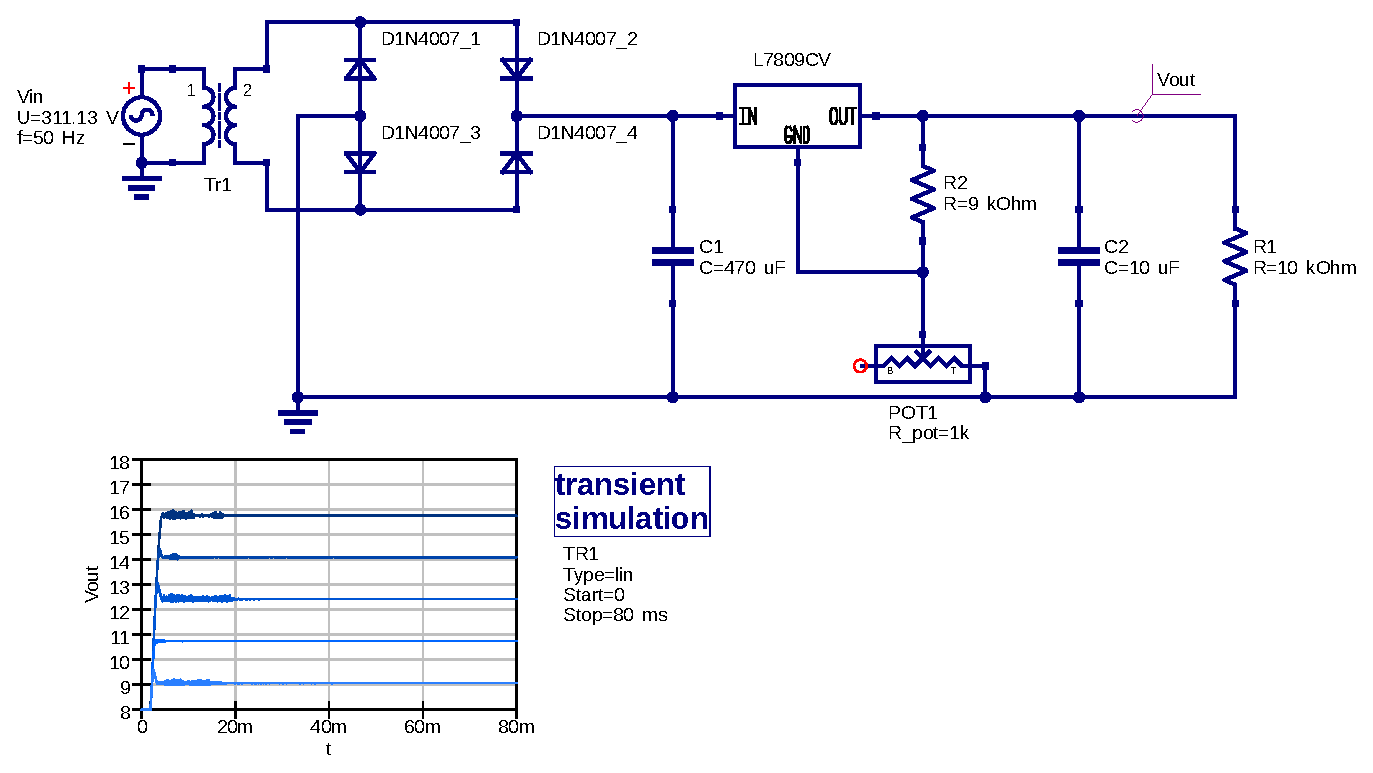
\includegraphics[scale=0.75]{simulacion/12.regulador4.eps}
\caption{Simulación del regulador variable con \textbf{L7809CV}.}
\label{simulacion12}
\end{figure}

\begin{figure}[!h]
\centering
\includegraphics[scale=0.28]{fotos/12.regulador4.eps}
\caption{Regulación variable con \textbf{L7809CV} \\
y medición de corriente y voltaje.}
\label{laboratorio14}
\end{figure}

\subsubsection{Laboratorio}
Se presenta el regulador \textbf{L7809CV} armado en laboratorio, así como su
voltaje y corriente en un multímetro para los valores de resistencia variable de
$0[\Omega]$ y $1[\text{k}\Omega]$, este puede verse en la
\textbf{figura~\ref{laboratorio14}}.

